\documentclass[10pt]{article}

\usepackage{spheric}
%%%TITLE
\title{The $\delta$ALE-SPH model: an improved $\delta$-SPH scheme containing particle shifting and ALE formulation}
\date{}

%%AFFILIATIONS

\author[1]{P.N. Sun$^\dagger$}
\author[1]{A.M. Zhang$^*$}

\author[2]{A. Colagrossi$^\ddag$}
\author[2]{S. Marrone}
\author[2]{ M. Antuono}

\affil[1]{College of Shipbuilding Engineering, Harbin Engineering University, Harbin, China}
\affil[2]{CNR-INSEAN, Marine Technology Research Institute, Rome, Italy}
 
\affil[$\relax$]{\email{\dagger}{sunpengnan@yeah.net}, \email{*}{zhangaman@hrbeu.edu.cn}, \email{\ddag}{andrea.colagrossi@cnr.it}}


%%DOCUMENT
\begin{document}

\maketitle

%\SelectedTopics{}

%%PLEASE PUT YOUR ABSTRACT HERE
\begin{abstract}
 In the present work we derive a novel model, named $\delta$ALE-SPH scheme, by merging the $\delta$+SPH scheme \cite{sun2017deltaplus} and the Arbitrary Lagrangian Eulerian (ALE) formulation \cite{oger2016sph}. Differently from the $\delta^+$SPH scheme, the use of the ALE framework allows for a consistent inclusion of the Particle Shifting Technique (PST) and, consequently, for recovering the conservation of mass and linear momentum. In the proposed scheme, a diffusive term is included in the density equations to ensure a regular pressure field. Furthermore, different constraints on the mass flux equation are investigated. Indeed we discovered that the accuracy of the solution as well as the properties of the scheme strongly depend on how this equation is numerically handled.
 
Suitable algorithms for the numerical treatment near the free surface and on the solid wall boundary are implemented. These treatments improve the particle distribution and the pressure evaluation close to the fluid boundary. Finally, the $\delta$ALE-SPH scheme is tested against several challenging benchmark test cases, proving to be more robust and accurate than the other SPH schemes. 

\begin{figure}[!htb]
\centering
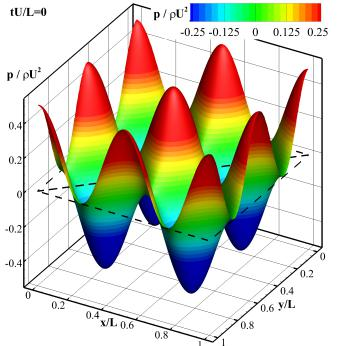
\includegraphics[width=0.24\textwidth]{40-11.png}
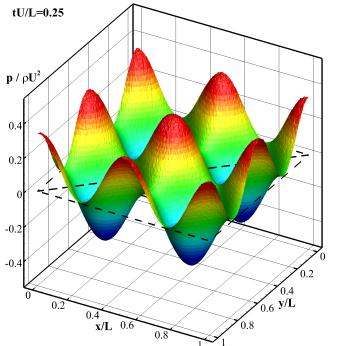
\includegraphics[width=0.24\textwidth]{40-12.png}
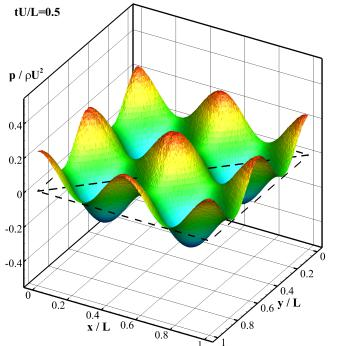
\includegraphics[width=0.24\textwidth]{40-13.png}
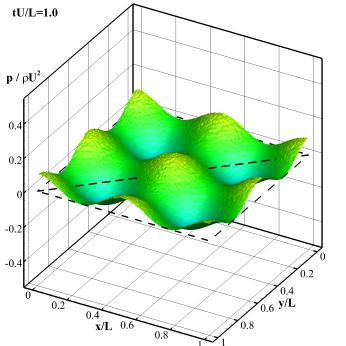
\includegraphics[width=0.24\textwidth]{40-14.png}
\caption{Pressure distribution on the fluid domain occupied by the Taylor Green vortices at four time instants when Re=100: the vertical axis shows the pressure amplitude and the two horizontal axes show the positions.}\label{fig:40-1}
\end{figure}

\begin{figure}[!htb]
\begin{minipage}[t]{0.3\linewidth}
\centering
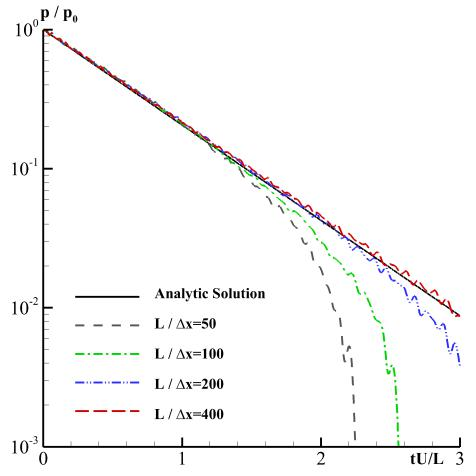
\includegraphics[width=0.95\textwidth]{40-2.png}
\caption{Time evolution of the pressure measured on the fluid center at Re = 100.}\label{fig:40-2}
\end{minipage}
\begin{minipage}[t]{0.05\linewidth}
~~
\end{minipage}
\begin{minipage}[t]{0.62\linewidth}
\centering
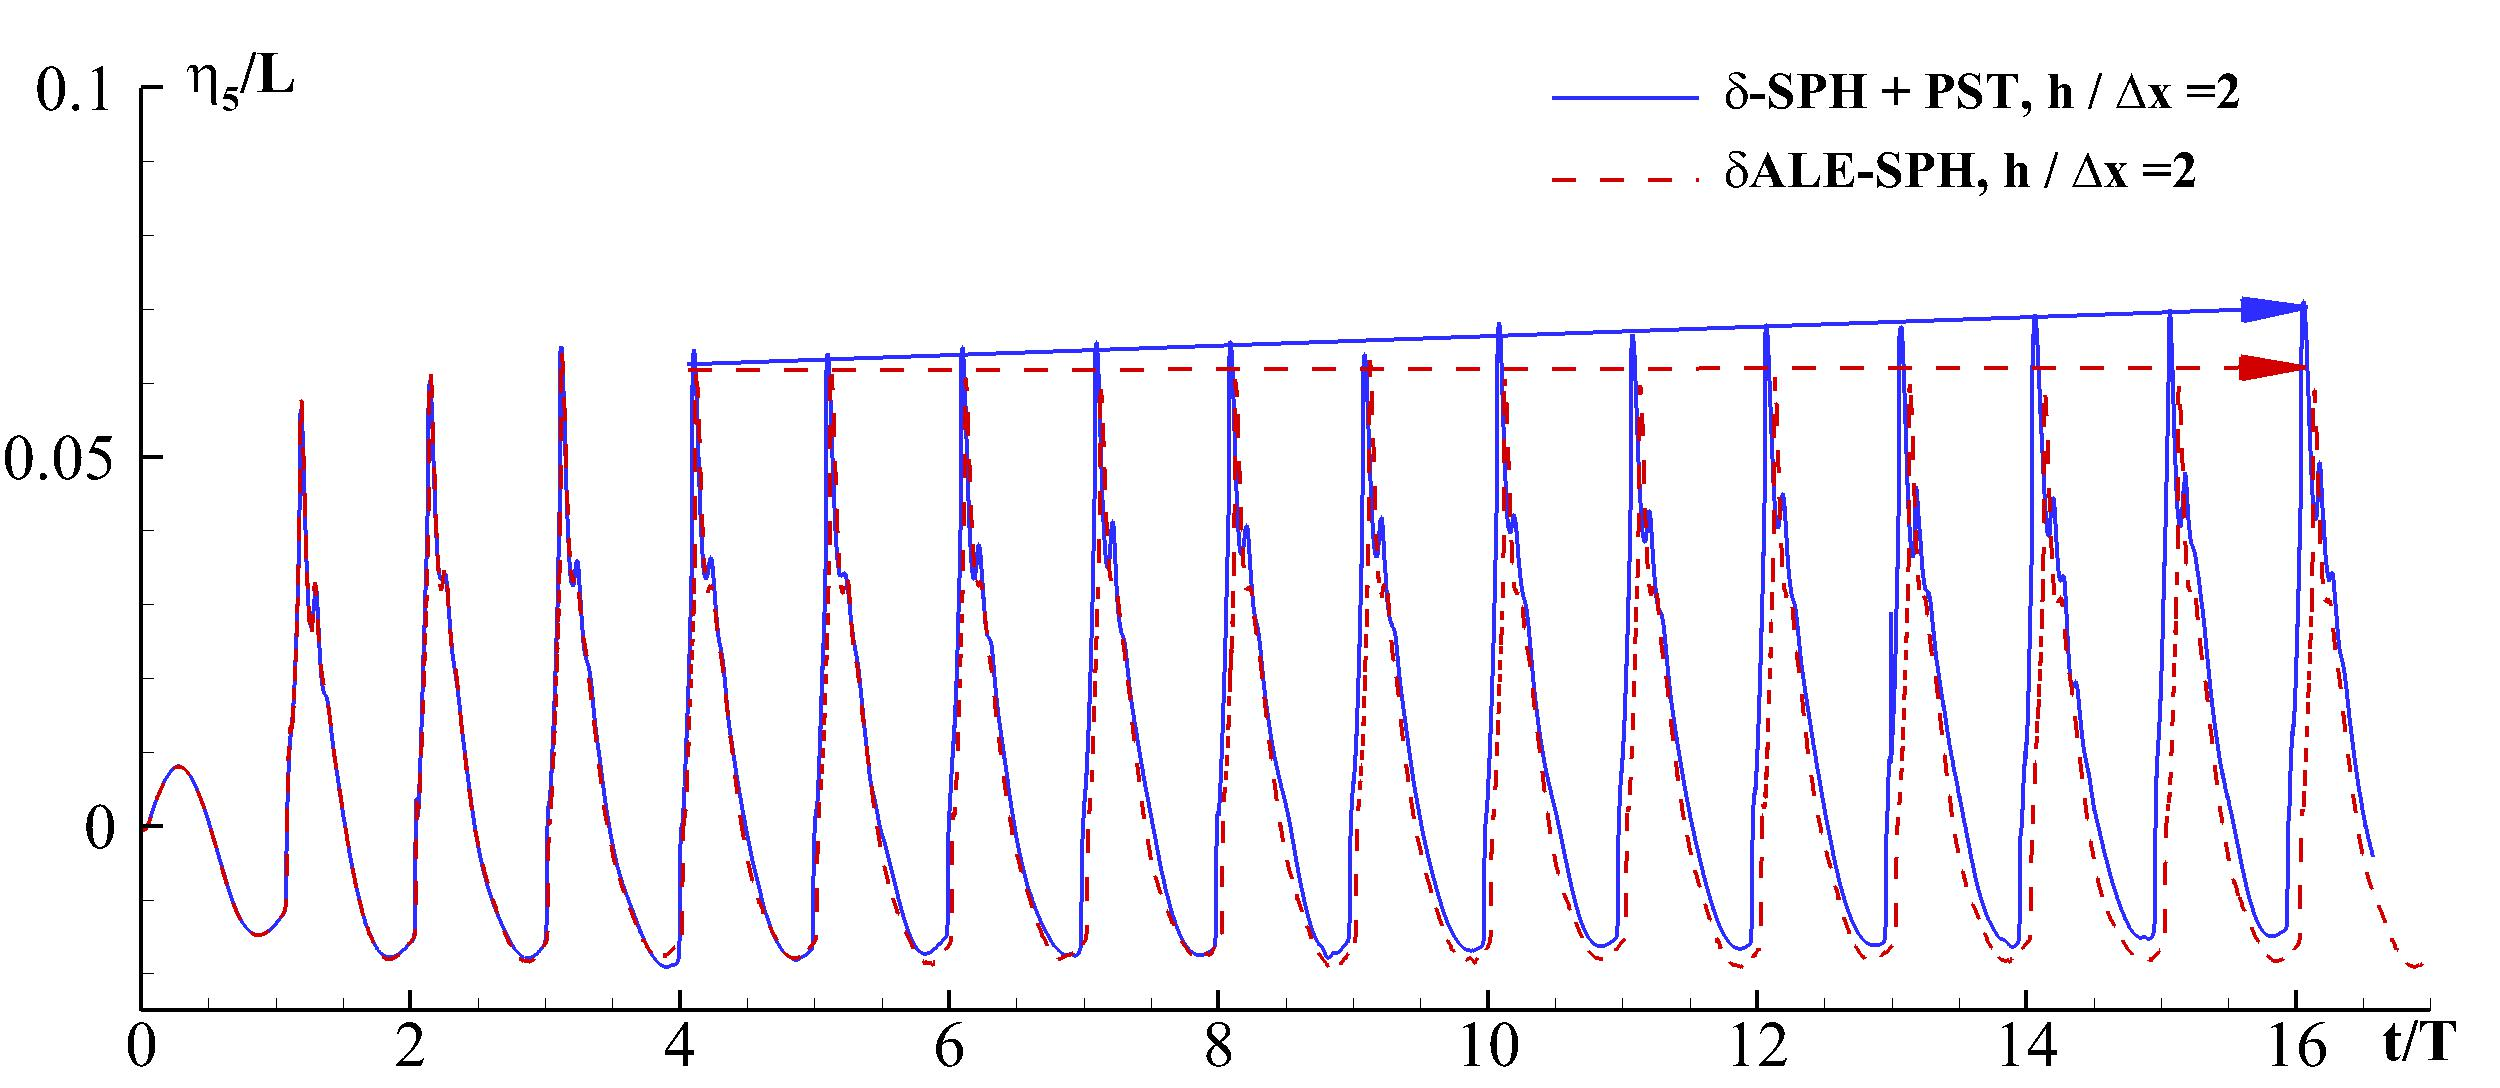
\includegraphics[width=\textwidth]{40-3.png}
\caption{Time evolution of the wave height measured on a fixed position in a sloshing tank with horizontal oscillations. Results between $\delta$ALE-SPH scheme and $\delta$-SPH with PST are compared.}\label{fig:40-3}
\end{minipage}
\end{figure}

Taking the benchmark test Taylor-Green Vortices as example, the pressure field at different time instants are depicted in Figure \ref{fig:40-1}. The absolute value of the pressure field gradually converges to zero (zero pressure is marked by the dashed plane in the four subplots in Figure \ref{fig:40-1}). The pressure evolutions measured on the center of the fluid are plotted in Figure \ref{fig:40-2} for four different particle resolutions which show a fair convergence of the results to the analytic solution. Another example is the sloshing test as shown in Figure \ref{fig:40-3}. The result of simply implementing PST in $\delta$-SPH shows a free surface rising up after a long time. The free surface rising up is mainly due to the non-conservation of momentum after the particle shifting. While in the result of $\delta$ALE-SPH, the maximum height of the free surface has been almost constant, see the red arrow in Figure \ref{fig:40-3}. Further numerical studies by other benchmarks will be presented in the full-length paper. 
\end{abstract}


%%THE END OF ABSTRACT

\addbib

\end{document}
